\chapter{Android}
	\minitoc
	\newpage
%%%%%%%%%%%%%%%%%%%%%%%%%%%%%%%%%%%%%%%%%%%%%%%%%%%%%%%%%%%%%%%%%%%%%%%%%%%%%%%%%%%%%%%%%%%%%
\section{Description}
Android est un système d'exploitation open source développé principalement par Google pour une variété de dispositifs, principalement les smartphones et les tablettes. Voici quelques points clés pour comprendre Android :
\begin{itemize}
\item[-]\textbf{Système d'exploitation mobile :} Android est un système d'exploitation conçu spécifiquement pour les appareils mobiles. Il offre un environnement informatique complet, incluant le système d'exploitation, le middleware et les applications de base. Android est basé sur le noyau Linux, ce qui lui confère une stabilité et une sécurité accrues.
\item[-]\textbf{Open Source :} Android est un projet open source, ce qui signifie que son code source est disponible et peut être modifié par les développeurs. Cela favorise la flexibilité, l'innovation et la collaboration. 
\item[-]\textbf{Écosystème d'applications :} L'une des caractéristiques distinctives d'Android est son vaste écosystème d'applications. Les développeurs peuvent créer des applications pour Android en utilisant le langage de programmation Java (ou Kotlin) et les distribuer via la plateforme Google Play Store.
\end{itemize}
	\begin{figure}[!h]
    	\center
    		
\includegraphics[width=0.5\textwidth]{image/android_logo.jpg}
   		\caption{Logo Android}
    	\label{Logo Android}
	\end{figure}

\subsection{Principale contrainte}
Le développement d'applications sous Android offre de nombreuses opportunités, mais il comporte également des défis et des contraintes. Voici quelques-unes des contraintes courantes associées au développement sous Android :
\begin{itemize}
   \item[-]\textbf{Fragmentation : }Comme mentionné précédemment, l'écosystème Android est fragmenté en raison de la diversité des fabricants, des modèles et des versions du système d'exploitation en circulation. Cela signifie que les développeurs doivent prendre en compte cette diversité lors de la conception et du test de leurs applications pour assurer une compatibilité optimale.
   \item[-]\textbf{Compatibilité des Appareils :} En raison de la diversité matérielle, certaines applications peuvent ne pas fonctionner de manière optimale sur tous les appareils Android en raison des variations de taille d'écran, de résolution, de puissance de traitement, etc.
\item[-]\textbf{Mises à Jour du Système d'Exploitation : } Les mises à jour d'Android ne sont pas toujours déployées uniformément sur tous les appareils, car cela dépend des fabricants et des opérateurs. Certains utilisateurs peuvent continuer à utiliser des versions plus anciennes d'Android, ce qui peut rendre difficile la prise en charge de certaines fonctionnalités récentes dans les applications.
    \item[-]\textbf{Sécurité :}   En raison de la nature open source d'Android, il peut être plus vulnérable aux attaques de sécurité que des systèmes plus fermés. Les développeurs doivent prendre des mesures supplémentaires pour sécuriser leurs applications et protéger les données des utilisateurs.
   \item[-]\textbf{Optimisation des Performances :} En raison de la diversité des dispositifs, il peut être plus complexe d'optimiser les performances des applications pour garantir une expérience utilisateur fluide sur toutes les plateformes.
    \item[-]\textbf{Distribution des Applications :}  Bien que la distribution via Google Play soit la méthode la plus courante, certains marchés et régions peuvent avoir des restrictions ou des préférences spécifiques en matière de distribution, ce qui peut poser des défis pour la portée globale de l'application.
    \item[-]\textbf{ Ressources Limitées :} Certains appareils Android peuvent avoir des ressources limitées en termes de mémoire, de puissance de traitement et de stockage. Les développeurs doivent optimiser leurs applications pour fonctionner efficacement sur une gamme variée de matériel.
\end{itemize}
\subsection{Couche d’android }
Le développement Android repose sur un ensemble de couches logicielles qui fournissent les fonctionnalités nécessaires pour créer des applications. Ces couches constituent l'architecture du système d'exploitation Android. Voici les principales couches d'Android, de la plus basse à la plus haute :
   \begin{itemize}
    \item[-]\textbf{Noyau Linux : } Android est construit sur le noyau Linux, qui fournit les fonctionnalités de base du système d'exploitation, telles que la gestion de la mémoire, la gestion des processus, la gestion du système de fichiers, et la communication avec le matériel.
    \item[-]\textbf{Bibliothèques Android :}  Cette couche comprend un ensemble de bibliothèques écrites en langage C/C++ qui sont utilisées par divers composants du système Android. Ces bibliothèques fournissent des fonctionnalités telles que la gestion des graphiques, l'accès à la base de données SQLite, la manipulation d'images, etc.
    \item[-]\textbf{Android Runtime (ART) :} Il s'agit de l'environnement d'exécution des applications Android. Il utilise le bytecode DEX (Dalvik Executable) pour exécuter les applications. À partir d'Android 5.0, ART a remplacé Dalvik comme moteur d'exécution par défaut.
    \item[-]\textbf{Framework d'Application : } Cette couche fournit les classes et les services nécessaires au développement des applications Android. Elle inclut des composants tels que les activités, les services, les fournisseurs de contenu, les gestionnaires d'applications, etc. Les développeurs utilisent ce framework pour construire l'interface utilisateur et la logique métier de leurs applications.
    \item[-]\textbf{Applications Système :}   Au sommet de la pile se trouvent les applications système préinstallées sur chaque appareil Android. Cela inclut des applications telles que le lanceur (interface utilisateur), le gestionnaire d'applications, le navigateur, le gestionnaire de contacts, etc. Ces applications offrent une expérience utilisateur de base et servent de référence pour les développeurs d'applications tierces.
    \end{itemize}
%%%%%%%%%%%%%%%%%%%%%%%%%%%%%%image couche android%%%%%%%%%%%%%%%%%%%%%%
	\begin{figure}[!h]
    	\center
    		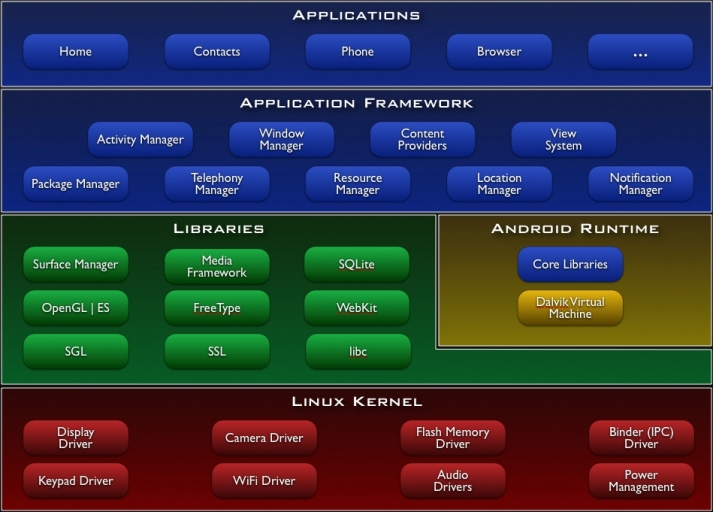
\includegraphics[width=0.8\textwidth]{image/318598}
   		\caption{Couche android}
    	\label{Couche android}
	\end{figure}
\section{Le langage Java}
Java est un langage de programmation de haut niveau, orienté objet et indépendant de la plateforme. Il a été créé par Sun Microsystems (maintenant une division d'Oracle) et a été rendu public en 1995.
\subsection{Les variables}
En informatique, les variables sont des symboles qui associent un nom à une valeur. Il existe deux types que l’on utilisera :\\
Type Primitive : Ce sont des types de donnée non objet qu'on retrouve dans de nombreux autres langages de programmation. A chacun de ces types correspond un type objet appelé «type enveloppe».\\
Ex : float,int \\
Objet : L'objet est comparable au tableau à la seule différence que chaque variable stockée n’est pas appelée par un index mais par un nom.\\
%%%%%%%%%%%%%%%%%%%%%%%%%code instanciation%%%%%%%%%%%%%%%%%%%
En Java, la déclaration d'une classe, d'une méthode ou d'un membre peut être précédée par un modificateur d'accès ou attribut.\\
Un modificateur indique si les autres classes de l'application pourront accéder ou non à la classe/méthode/membre 
Une classe a une visibilité :
\begin{itemize}
\item[-]\textbf{public:}  sa définition est précédée de public, et il peut être utilisé par tout utilisateur de la classe.
\item[-]\textbf{privé:} sa définition est précédée de private, et il ne peut être utilisé qu’à l’intérieur de la classe
\item[-]\textbf{protégé:} sa définition est précédée de protected, et il ne peut être utilisé qu’à l’intérieur de la classe, ou des classes dérivées.
\item[-]\textbf{paquetage:} l’attribut peut être utilisé dans toute classe du même paquetage.
\end{itemize}
par défaut : sans modificateur d'accès, seules les classes du même package peuvent accéder à l'item.\\
Il y a aussi d’autre attribut pour les variable type objet comme :
\begin{itemize}
\item[-]\textbf{Abstract :} une classe abstraite est une classe dont l'implémentation n'est pas complète et qui n'est pas instanciable. Elle sert de base à d'autres classes dérivées (héritées).
\item[-]\textbf{final:} indique qu'un élément ne peut être changé dans la suite du programme.
\item[-]\textbf{Static:} Une méthode statique est une méthode qui peut être appelée même sans avoir instancié la classe.
\end{itemize}
\subsection{Compilation}
Un compilateur Java est un compilateur pour le langage de programmation Java. Le format de sortie le plus courant pour un compilateur Java est des fichiers .class contenant le bytecode Java plate-forme agnostique. Il existe aussi des compilateurs produisant du code machine optimisé pour une combinaison matériel/système d'exploitation particulière.\\
La machine virtuelle Java (JVM) charge les fichiers .class et interprètes le bytecode ou le compile à la volée et peut également l'optimiser en utilisant la compilation dynamique.\\
Ainsi on utilise un Java Devellopement Kit(JDK) ou on peut trouver JRE(Java Runtime Environnement ) contient JVM (Java virual Machine ) .\\
Exploiter une nouvelle plate-forme n’est jamais chose aisée. C’est pourquoi Google fournit, en plus du système d’exploitation, un kit de développement .Ce SDK est un ensemble d’outils logiciels qui permet aux développeurs et aux entreprises de créer des applications.\\
Un kit de développement logiciel, aussi appelé trousse de développement logiciel, facilite donc  le développement d'un logiciel sur une plateforme donnée.\\
Et aussi d’un API qui est un ensemble de classes regroupant des fonctions mises à disposition des développeurs. Ces fonctions ou méthodes peuvent être regroupées dans des bibliothèques logicielles ou des services. Le plus souvent, elles effectuent des traitements de bas niveau et proposent au développeur une interface de plus haut niveau pour qu’il puisse accéder à des fonctionnalités plus facilement et surtout plus immédiatement.\\
La forme de paquet SDK est :
\textbf{Android[nombre](API[un autre nombre])}\\
Cette SDK  est aussi suivi d’un ADT(Android Devellopment Tools) qui ajoute le support intégré pour Android projets et des outils. Le plugin ADT comprend une variété d'extensions puissantes qui font création, l'exécution et le débogage Android des applications plus rapidement et plus facilement.\\
%%%%%%%%%%%%%%%%%%%%%%%%%compile
	\begin{figure}[!h]
    	\center
    		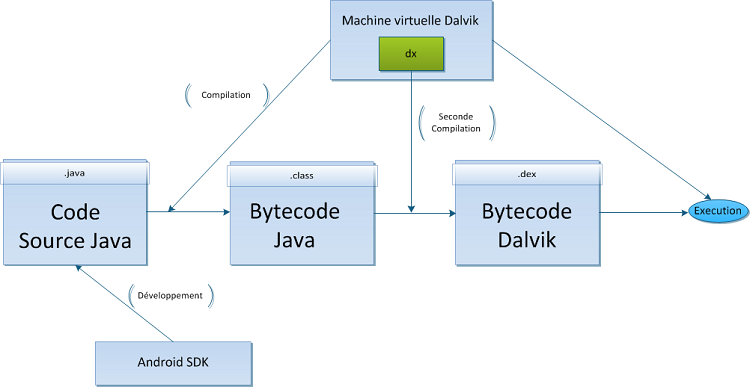
\includegraphics[width=0.8\textwidth]{image/compile}
   		\caption{Compilation}
    	\label{Compilation}
	\end{figure}
\section{Composition de fichier}
Donc un projet et généralement composer de :\\
\textbf{R.java:} Fichier contenant les "paramètres" de l'application. Il se génère automatiquement.\\
\textbf{Bin:} : Le dossier "Bin" contient les binaires de l'application \\
\textbf{Manifest :} description de l’application\\
\textbf{src\ :}  les fichiers source, une fois compiler  R.java est créé qui fournira des infos res\\
\textbf{libs :} bibliothèque\\
\textbf{res :} Ce dossier contient les ressource, les images utilisées dans le projet, les XML du projet (les fichiers XML servent à définir l'interface de l'application) et le dossier "values".\\
Généralement dans les ressources il y a :
\begin{itemize}
\item[-]ressource :xml
\item[-]Drawable
\item[-]Layout
\item[-]Menu
\item[-]Mipmap
\item[-]Value
\item[-]image accessible par R
\end{itemize}
\textbf{gen :} fichier par ADT(Android develloppment tools)\\
\textbf{assets/ :} ressource brutes (rawbytes) accessible par flux de donner \\
\textbf{andrid Manifest.xml :} décrivent l’application, fichier XML dans lequel on déclare les différentes activités de l'application, et certains paramètres de l'application (par exemple si on autorise la rotation de l'application, le sens de l'application (vertical, horizontal), l'icône de l'application, etc..).\\
\textbf{default.propretie :} propriété pour la compilation \\
\subsection{Gestion de ressource}
Langage de balisage est un langage qui s'écrit grâce à des balises. Ces balises permettent de structurer de manière hiérarchisée et organisée les données d'un document. Ici l’application utilise le xml.
\textbf{res/ :} stockage des ressource pour s’adapté au divers changement
\begin{lstlisting}
//debut de fichier
<?xml version="1.0" encoding="utf-8" ?>
\end{lstlisting}
Il y a des nœud parents et enfant
\textbf{res/drawable :} Ces dossiers contiennent les images ou les images matricielles de l'application. Tous ces dossiers devraient, dans l'idéal, contenir les mêmes images, mais avec des résolutions différentes. En effet, selon la résolution de l'écran utilisé, les images seront tirées du dossier correspondant.\\
\textbf{res/value :} ce dossier contient aussi des XML, mais qui servent à stocker des chaînes de caractères.\\
\textbf{res/layout :} Ce dossier contient les XML de l'application pour les interfaces. Vous pouvez déjà voir le main.xml, qui correspond à l'interface de l'activité principale de l'application.\\
\textbf{res/menu :} XML, menu\\
\textbf{res/raw :} données brute\\
\textbf{res/value :} catégorie nombreuse \\
	Ex : variable\\
la forme générale est donc:
\begin{lstlisting}
< ?xml version="1.0" encoding="utf-8"?>
<racine>
	< !--commentaire-->
	<elements 	attribut1="valeur 1"
attribut2="valeur 2">
<feuille1 attribut3="valeur 3"/>
<feuille2> texte </feuille2>
	</element>
</racine>
\end{lstlisting}
\subsection{Les quantificateur}
Les  quantificateurs  sont utilisés  pour cibler précisément un certain nombre de priorités  ; à savoir la langue et la région, la taille de l'écran, l'orientation de l'écran, la résolution de l'écran et la vers ion d'Android Les  restrictions  sont représentées  par des  quantificateurs  et ce sont ces  quantificateurs  qui vous  permettront de préciser le matériel pour lequel les fichiers  dans  ce répertoire sont destinés. La syntaxe à respecter peut être représentée ainsi :
\begin{lstlisting}
res/<type_de_ressource>[<-quantificateur 1><-quantificateur 2>...<-quantificateur N>]  
\end{lstlisting}
langue et région priorité 2 ex :fr\\
taille de l’écran :priorité :3 small,nomal,large,xlarge\\
orientation de  l’écran priorité :5 port,land\\
résolution de l’écran  priorité 8 :	
\begin{itemize}
\item[-]ldpi, 120dpi
\item[-]mdi 160 dpi
\item[-]hdmi 240dpi
\item[-]xhdpi 320dpi
\item[-]nodpi non redimensionee
\end{itemize}

Version d’Android priorité 14
ordre des priorité a respect croissante 
\section{Environnement de développement }
Grade script : outil de compilation\\
logCat :   message détailler debugge, info, erreur….\\
\begin{lstlisting}
	Log.i(String tag,String message)
	Log.w(tag,message)
	Log.e(tag,message)
\end{lstlisting}
ADB : Android Debugge Bridge passerelle PC et devise gestion serveur :\\
-adb start-server : démarre\\
-adb kill-server : arrêt\\
-adb device : liste des connectées\\
\subsection{Générer de paquet}
Build>generate Signed APK\\ 
Clé privé\\
Pour avoir une clé privée il faut un key store\\
Cree un key store :\\
Remplir\\
Cree clé privée\\
%%%%%generer paquet a expliquer avec image
%%%%%%%%%%%%%%%%%%%%%%%%%%image de cle%%%%%%%%%%%%%%%%%%%%%%%
Emplacement du fichier 
\subsection{Classe R} 
Classe R
La classe R se trouve :\\
App>build>generated>source>r>debug\\

Drawable :\\
Sting :\\
Pour récupérer les sources\\
Private String variable=null ;\\
Variable =getResource().getString(R.String.hello) ;
\textbf{Norme de nom}\\
Android : nom attribut\\
Il est possible de créer une interface par codage mais vaut mieux le stocker dans res/layout/main.xml, mettre chaque type dans le dossier qui le convient\\
Ex :string  res/value/strings.xml\\
@id/nom : utilise R.id.nom référence définit ailleurs\\
@+id/nom crée cet identifiant	\\
\subsection{Les composants}
Vue : élément de l’interface graphique\\ 
Contrôles : sous-ensemble de vue\\
Activité : écran structure \\
	ex : des vue a l’intérieur d’un vue\\
Xml : fichier de configuration \\
forme générale de fichier class d'une application
\begin{lstlisting}
Package projet.memoire.package ;
Import android.os.bundle ;
Import android.view.menu ;
Import android.view.MenuItem ;
Import androoid.support.V4.app.navutils ;
Public class MainActivity extends Activity{
	@Override //facultative
	Public void onCreate(bundle saveInstanceState){
		Super.oncreate(svedInstanceState) ;
setContentView(R.layout.activity_main) ;
}
@override//indique la redefinition de methode
Public boolean oncreateOptionMenu(Menu menu) {
	getMenuInflater().inflate(R.menu.activity_main,menu) ;
return true ;
}
}
\end{lstlisting}
Les ressource
Nous pouvons distinguer plusieurs types de ressources :
\begin{itemize}
\item[-]les fichiers de ressources de l'application (images, chaînes de caractères, layout, xml) qui dépendent du contexte (langue française, taille de l'écran, mode portrait/paysage…) ;
\item[-]les bases de données ;
\item[-]les fichiers préférences ;
\item[-]les fichiers pour la lecture et la lecture/écriture sans contexte.
\end{itemize}
\section{Pattern d'Android }
MVC (Modèle-Vue-Contrôleur) : Dans le modèle MVC, le code est organisé en trois composants principaux :
\begin{itemize}
    \item[-]\textbf{Modèle :} Représente la logique métier et les données de l'application.
    \item[-]\textbf{Vue : }Affiche l'interface utilisateur et interagit avec l'utilisateur.
    \item[-]\textbf{Contrôleur : } Gère les interactions de l'utilisateur, manipule les données du modèle et met à jour la vue.
\end{itemize}strucbasique
Dans le contexte Android, l'activité peut être considérée comme le contrôleur, la vue est l'interface utilisateur (XML) et le modèle est généralement représenté par des classes qui gèrent les données de l'application.

	\begin{figure}[!h]
    	\center
    		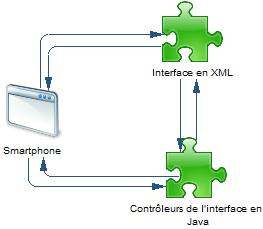
\includegraphics[width=0.5\textwidth]{image/strucbasique.jpg}
   		\caption{MVC Android}
    	\label{MVC Android}
	\end{figure}
	
\section{Conclusion}
Pour développer sur Android  il faut plusieurs élément, pour combler ses élément on utilise le SDK approprié pour faire apparaitre les éléments voulu par la version voulu du point de vue générale, on a besoin tout simplement des ressource, de la classe R et d’un Model. Et on constate que le développement d’Android et totalement dans le monde de MVC.


















